%%%%%%%%%%%%%%%%%%%%%%%%
%
% $Autor: Kreetika Mohanta$
% $Datum: 2025-06-11 20:48:02Z $
% $Pfad: BA25-02-Time-Series/report/Contents/en/ApplicationAppendix.tex
% $Version: 4621 $
%
% !TeX encoding = utf8
% !TeX root = Rename
%
%%%%%%%%%%%%%%%%%%%%%%%%

\chapter{Bill of Materials}

\section{Material List and Hardware Bill of Materials}

The following hardware components were used for developing, testing, and running the hurricane intensity prediction system.

\begin{table}[H]
	\centering
	\renewcommand{\arraystretch}{1.2}
	\begin{tabular}{|>{\centering\arraybackslash}m{3.8cm}|m{3.5cm}|m{1.4cm}|m{3.2cm}|m{2cm}|}
		\hline
		\textbf{Materials} & \textbf{Description} & \textbf{Qty} & \textbf{Link} & \textbf{Price} \\
		\hline
		
		\makecell{\rule{0pt}{2.5cm}
\includegraphics[width=2.8cm]{../../BA25-02-Time-Series/report/Images/Laptop.PNG}} &
		Lenovo LOQ Gen 9 used for model training, analysis, and Streamlit UI. &
		1 &
		\href{https://www.lenovo.com/de/de/p/laptops/loq-laptops/lenovo-loq-essential-gen-9-15-intel/83lkcto1wwde1}{Link} &
		591.75 € \\
		\hline
		
		\makecell{\rule{0pt}{2.5cm}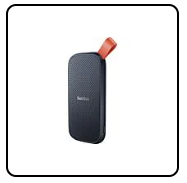
\includegraphics[width=2.8cm]{../../BA25-02-Time-Series/report/Images/HardDrive.PNG}} &
		SanDisk 1TB SSD for storing datasets, models, and backups. &
		1 &
		\href{https://www.mediamarkt.de/de/product/_sandisk-portable-usb-32-gen-2-speicher-1-tb-ssd-extern-schwarz-2881031.html}{Link} &
		79.99 € \\
		\hline
	\end{tabular}
	\caption{Hardware Bill of Materials}
	\label{tab:hardware}
\end{table}


\begin{figure}[H]
	\centering
	
\includegraphics[width=0.5\textwidth]{../../BA25-02-Time-Series/report/Images/Laptop.PNG}
	\caption{Lenovo LOQ Essential Gen 9}
\end{figure}

\begin{figure}[H]
	\centering
	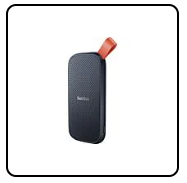
\includegraphics[width=0.5\textwidth]{../../BA25-02-Time-Series/report/Images/HardDrive.PNG}
	\caption{SanDisk 1TB SSD}
\end{figure}

\newpage

\section{Software Requirements and Python Libraries}

\begin{table}[H]
	\centering
	\renewcommand{\arraystretch}{1.5}
	\begin{tabular}{|m{3.5cm}|m{5.5cm}|m{3.5cm}|m{1.8cm}|}
		\hline
		\textbf{Software / Library} & \textbf{Description} & \textbf{Platform / Interface} & \textbf{Cost} \\
		\hline
		Python & Main language for development and modeling. & VS Code, Jupyter & Free \\
		\hline
		Streamlit & Web framework used to build a user-friendly UI for predictions. & Browser UI & Free \\
		\hline
		scikit-learn & For error metrics (MAE, RMSE), splitting, and preprocessing. & Python Library & Free \\
		\hline
		statsmodels & Used for ARIMA implementation and time series handling. & Python Library & Free \\
		\hline
		tensorflow + keras & Used for building and training LSTM models. & Python Library & Free \\
		\hline
		joblib & For saving and loading trained models (serialization). & Python Utility & Free \\
		\hline
		matplotlib, plotly & For static and interactive visualization of trends and predictions. & Python Visualization Tools & Free \\
		\hline
		pandas, numpy & For data cleaning, manipulation, time series indexing, and numerical ops. & Python Core Libraries & Free \\
		\hline
		requests & Enables HTTP requests (for future API support). & Python Library & Free \\
		\hline
		LaTeX & Used to write this manual. & TeXstudio & Free \\
		\hline
	\end{tabular}
	\caption{Software and Libraries Used}
	\label{tab:software}
\end{table}
\newpage
\section{requirements.txt}

The following Python packages were essential for executing the entire hurricane intensity forecasting pipeline:

\begin{lstlisting}[language=Python, caption={requirements.txt}]
	streamlit
	pandas
	numpy
	joblib
	keras
	tensorflow
	statsmodels==0.13.5
	scikit-learn
	matplotlib
	plotly
	requests
\end{lstlisting}

\section{Explanation of Key Libraries}

\begin{itemize}
	\item \textbf{pandas, numpy} – Handle dataset loading, cleaning, transformations, and numerical operations.
	\item \textbf{scikit-learn} – For calculating evaluation metrics (e.g., MAE, RMSE), scaling, and data preprocessing.
	\item \textbf{statsmodels} – Implements the ARIMA time series forecasting algorithm.
	\item \textbf{keras + tensorflow} – Used to build, train, and validate the LSTM deep learning model.
	\item \textbf{matplotlib + plotly} – Generate side-by-side visual comparisons of predicted vs actual hurricane intensities.
	\item \textbf{streamlit} – Provides a clean web interface where users can upload data and view model outputs interactively.
	\item \textbf{joblib} – Saves and reloads model states, enabling fast deployment and reproducibility.
	\item \textbf{requests} – Facilitates web-based data interactions (for future integration of APIs).
\end{itemize}

